\documentclass[10pt, xcolor=x11names]{beamer}
\usecolortheme{seagull}
\useoutertheme{infolines}
\usefonttheme[onlymath]{serif}
\setbeamertemplate{headline}[default]
\setbeamertemplate{navigation symbols}{}
\mode<beamer>{\setbeamertemplate{blocks}[rounded][shadow=true]}
\setbeamercovered{transparent}
\setbeamercolor{block body example}{fg=blue, bg=black!20}

\usepackage[utf8]{inputenc}
\usepackage[]{csquotes}
\usepackage{amsmath}
\usepackage{tikz, wasysym}
\usepackage{graphicx}
\usetikzlibrary{automata,positioning}
\usepackage{hyperref}
\usepackage{amsfonts}
\usepackage{csquotes}
\usepackage{tikz}
\usetikzlibrary{arrows}
\usetikzlibrary{arrows.meta}
\usepackage{wrapfig}
\usepackage{pgfplots}
\usepackage{outlines}


%\usepackage{amsfonts}
%\usepackage{amssymb}
%\usepackage{makeidx}
%\usepackage{graphicx}


\usepackage{hyperref}
\author{Sven Fiergolla}
\title[Colloquium]{Improving Run Length Encoding through preprocessing}
\subtitle[short version]{}
\date{14. Januar 2020}
%\institute[Uni Trier]{Universität Trier}
%\logo{\includegraphics[scale=.25]{unilogo.pdf}}

%read the data to \dataA
	


\begin{document}

	
	
	\frame{\maketitle}
	\frame{\frametitle{}
	\tableofcontents
	}



\section{Introduction}	
\frame{\frametitle{Introduction - A Bit of History}
	  \begin{itemize}
		\item rise of multimedia
		\item rise of the World Wide Web
		\item ever increasing data transfer
	\end{itemize}

\medskip 

  \begin{itemize}
	\visible<2->{  \item compress to save storage space \& to handle new types and volumes of data}
\end{itemize}	
}

\frame{\frametitle{Introduction - The Situation Today}
	\begin{itemize}
		\item burst of sensors and IoT
		\item massive and rapid increasing data transfer
	\end{itemize}
	
	\medskip 
	
	\begin{itemize}
		\visible<2->{  \item compress to lower transmission cost / time
		\item compress to handle increasing resolution, fidelity, dynamic range
		\item compression for cold archiving}
	\end{itemize}	
}

\section{Basics}
\frame{\frametitle{Basics of Compression}
	\begin{itemize}
		\item Non random data contains redundant information
		\item Compression is about pattern or structure identification and exploitation
		
		\visible<2->{  \item No algorithm can compress all possible data of a given length, even by one byte (Kolmogorov Complexity)}
	\end{itemize}	
}

\frame{\frametitle{Basics of Compression - Entropy Encoding}
	\begin{itemize}
		\item generating a probability model for the data
		\item compute variable length codes
		
		\visible<2->{ \item low speed, high compression strength
		\item recommended for poorly structured data}
	\end{itemize}	
}

\frame{\frametitle{Basics of Compression - Entropy Encoding}
\begin{outline}
		\1 Huffman Encoding (1952)
		\2 computes optimal length prefix-free codes for symbols acc. to their probabilities
		\visible<2->{ \1 Run Length Encoding (1967) \2 computes runs of identical symbols}
		\visible<3->{ \1 Arithmetic Encoding (1979) \2 encodes a message of symbols in a single rational number in [0,1]}
		\visible<4->{\1 Asymmetric Numeral Systems (ANS) Encoding (2014) \2 encodes a message of symbols in a single natural number}
\end{outline}
}

\frame{\frametitle{Run Length Encoding (RLE)}
	\begin{outline}
\1 employed in the transmission of analog television signals as far back as 1967
\1 particularly well suited to palette-based bitmap images such as computer icons
\end{outline}
}

\frame{\frametitle{Run Length Encoding}
\[
aaaaabbbbbbaaaaaabb
\]
\visible<2->{
\[
a^5b^6a^6b^2
\]}
}

\frame{\frametitle{Run Length Encoding}
	\[
	aabaabbabbbababaabb
	\]
	\visible<2->{
		\[
		a^2b^1a^2b^2a^1b^3a^1b^1a^1b^1a^2b^2
		\]}
}

\frame{\frametitle{Huffman Encoding}
	\begin{figure}[h]
		\centering
		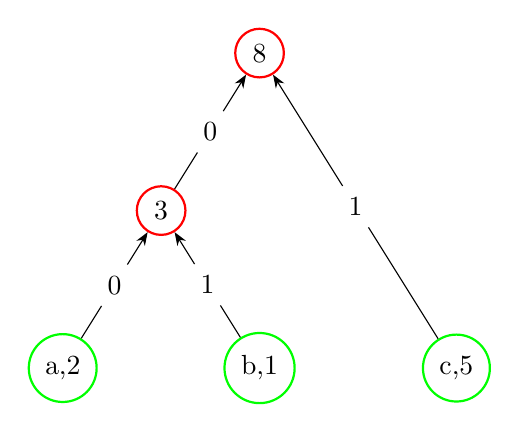
\begin{tikzpicture}
		\begin{scope}[every node/.style={circle,thick,draw=red}]
		\visible<2->{\node (B) at (1.25,2) {3};}
		\visible<3->{\node (C) at (2.5,4) {8};}
		\end{scope}
		\begin{scope}[every node/.style={circle,thick,draw=green}]
		\node (A) at (0,0) {a,2};
		\node (D) at (2.5,0) {b,1};
		\node (F) at (5,0) {c,5} ;
		\end{scope}
		
		\begin{scope}[>={Stealth[black]},
		every node/.style={fill=white,circle}]
		\visible<2->{\path [->] (A) edge node {$0$} (B);}
		\visible<3->{\path [->] (B) edge node {$0$} (C);}
		\visible<2->{\path [->] (D) edge node {$1$} (B);}
		\visible<3->{\path [->] (F) edge node {$1$} (C);}
		
		\end{scope}
		\end{tikzpicture}
		\caption{Example Huffman tree with 3 leaf nodes.} \label{fig:M1:example Huffman tree}
	\end{figure}
}


\frame{\frametitle{Basics of Compression - Dictionary Encoding}
	\begin{outline}
		\1 maintain a dictionary of strings for either a \emph{sliding window} or the whole data
		\2 replace later occurrence with reference position an length
		\visible<2->{ \1 High speed, moderate compression strength}
		\visible<3->{ \1 Famous Lempel-Ziv methods LZ77 and LZ78 (1977/78) \2 many derivatives, some still used today}
	\end{outline}
}

\frame{\frametitle{State of the art}
	\begin{table}[h]
	\begin{tabular}{r|r|r|r|r}
		method & options &  size in bytes & compression & \textit{bps}\\
		\hline
		uncompressed & & 3,145,718 & 100.0\% & 8.00 \\
		compress 4.2.4 & & 1,250,382 & 40.4\% & 3.24 \\
		gzip v1.10 & -9 & 1,021,720 & 32.4\% & 2.60\\
		ZIP v3.0 &-9& 1,019,783 & 32.4\% & 2.59 \\
		zstandard 1.4.2& --ultra-23 -long=30 & 887,004 & 28.1\% & 2.25\\
		bzip2 v1.0.8 & --best & 832,443 & 26.4\% & 2.11 \\
		brotli 1.0.7 & -q 11 -w 24 & 826,638 & 26.3\%& 2.10\\
		p7zip 16.02 (deflate) & a -mx10 & 821,873 & 26.1\% & 2.08 \\
		p7zip 16.02 (PPMd) & a -mm=ppmd o=32 & 763,067& 24.2\% & 1.93 \\
		ZPAQ v7.15 & -m5 & 659,700 & 20.9\% & 1.67  \\
		paq8hp* & - & - & - & - \\
		cmix v18 & -c -d & 554,983 & 17.6\% & 1.41 		
	\end{tabular}
	\label{tab:t20 stat of the art}
	\caption{State of the art compression ratios on the Calgary Corpus.}
\end{table}
}


\section{Design}
\frame{\frametitle{Design}
	
}

\frame{\frametitle{Design - Calgary Corpus}
	\begin{table}[H]
		\centering
		\begin{tabular}{l|r|l}	
			file & size & description\\
			\hline
			bib & 111261 & ASCII text - 725 bibliographic references\\
			book1 & 768771 & unformatted ASCII text\\
			book2 & 610856 & ASCII text in UNIX \enquote{troff} format\\
			geo & 102400 & 32 bit numbers in IBM floating point format\\
			news & 377109 & ASCII text - USENET batch file on a variety of topics\\
			obj1 & 21504 & VAX executable program \\
			obj2 & 246814 &	Macintosh executable program \\
			paper1 & 53161 & UNIX \enquote{troff} format \\
			paper2 & 82199 & UNIX \enquote{troff} format \\
			pic & 513216 & 1728 x 2376 bitmap image\\
			progc & 39611 & Source code in C \\
			progl & 71646 &  Source code in Lisp\\
			progp & 49379 & Source code in Pascal\\
			trans & 93695 & ASCII and control characters\\	 
		\end{tabular}
		\caption{The Calgary Corpus.}
		\label{tab:t05 The Calgary Corpus}
	\end{table}	
}

\frame{\frametitle{Design - Unmodified compression}
\begin{table}[h]
	\centering
	\begin{tabular}{l|r|r||r|r}
		bits per rle number & \multicolumn{2}{c}{byte-wise RLE} & \multicolumn{2}{c}{binary RLE} \\
		 &  ratio in \% & \textit{bps} & ratio in \% & \textit{bps}\\
		\hline
		8 & 165 & 13.20 & 329 & 26.38\\
		7 & 154 & 12.38 & 288 & 23.11\\
		6 & 144 & 11.57 & 248 & 19.87 \\
		5 & 134 & 10.77 & 208 & 16.66\\
		4 & 125 & 10.00 & 168 & 13.51\\
		3 & 116 & 9.29 & 131 & 10.50\\
		2 & 109 & 8.74 & 104 & 8.36
	\end{tabular}
	\caption{Byte-wise RLE on the Calgary Corpus.}
	\label{tab:t31 Byte-wise RLE on the Calgary Corpus}
\end{table}
}

\frame{\frametitle{Design - Unmodified compression}
\begin{table}[H]
	\centering
	\begin{tabular}{r|r|r|r|r|r}	
		file & size original & $\frac{bits}{\text{RLE number}}$ & size encoded & ratio in \% & \textit{bps}\\
		\hline
		pic & 513216 & 2 & 350292 & 68.25 & 5.46 \\
		& & 3 & 235067 & 45.80 & 3.66\\
		& & 4 & 165745 & 32.29 & 2.58\\
		& & 5 & 126349 & 24.61 & 1.96\\
		& & 6 & 106773 & 20.80 & 1.66\\
		& & 7 & 100098 & 19.50 & 1.56\\
		& & 8 & 101014 & 19.68 & 1.57\\		 
	\end{tabular}
	\caption{The file \textit{pic} with increasing bits per binary RLE encoded number.}
	\label{tab:t40 The file pic with increasing bits per RLE encoded number}
\end{table}	
\begin{itemize}
	\visible<2->{\item Byte-wise RLE achieves $27.2\%$ of its original size using 2.17 \textit{bps}.}
\end{itemize}
}

\frame{\frametitle{Design - Preprocessing}
	\begin{outline}
		\1 Most files other than pallet based images do not contain long runs of identical bit values.
		\visible<2->{\1 Files with long runs work really well with RLE.}
		\medskip
		\visible<3->{\1 Artificially creating runs on arbitrary data will improve the performance of RLE.}
	\end{outline}	
	}
	
\frame{\frametitle{Preprocessing}
	\begin{outline}
		\1 Vertical interpretation of the input
		\visible<2->{\1 Dynamic byte remapping}
		\visible<3->{\1 Burrows-Wheeler-Transformation}
		\visible<4->{\1 Huffman Encoding of runs}
	\end{outline}	
}

\frame{\frametitle{Preprocessing - Vertical interpretation}
	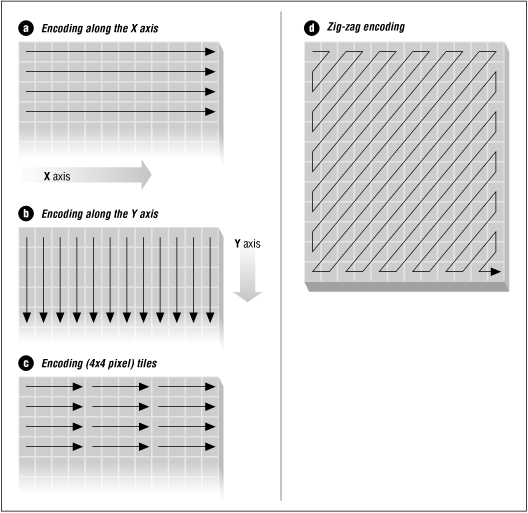
\includegraphics[height=\textheight, width=\textwidth]{g0902.png}
}

\frame{\frametitle{Preprocessing - Vertical interpretation}
		TODO: show 1d and 2d data
	}


\frame{\frametitle{Preprocessing - Vertical interpretation}
	TODO: show byte remapping
}


\frame{\frametitle{Preprocessing - Burrows-Wheeler-Transformation}
	
}

\frame{\frametitle{Preprocessing - Burrows-Wheeler-Transformation}
	
	\[
		S = abcabr
	\]
	
		\only<1>{
			\begin{table}[h]
				\centering
				\begin{tabular}{r|l|l|l|l|l|l}
					row 1 & a & b & c & a & b & r\\
					\hline
					row 2 & r & a & b & c & a & b\\	
					\hline
					row 3 & b & r & a & b & c & a\\
					\hline
					row 4 & a & b & r & a & b & c\\
					\hline
					row 5 & c & a & b & r & a & b\\
					\hline
					row 6 & b & c & a & b & r & a
						\label{tab:t10 bwt-example1}
				\end{tabular}
				\caption{Burrows Wheeler Transformation Matrix (all cyclic rotations).}
			\end{table}
		}
	\only<2>{
	\begin{table}[h]
		\centering
		\begin{tabular}{r|l|l|l|l|l|l}
			row 1 & a & b & c & a & b & r\\
			\hline
			row 2 & a & b & r & a & b & c\\
			\hline
			row 3 & b & c & a & b & r & a\\
			\hline
			row 4 & b & r & a & b & c & a\\
			\hline
			row 5 & c & a & b & r & a & b\\
			\hline
			row 6 & r & a & b & c & a & b	
			\label{tab:t10 bwt-example2}
		\end{tabular}
		\caption{Burrows Wheeler Transformation Matrix (all cyclic rotations, sorted).}
	\end{table}
}
}

\frame{\frametitle{Preprocessing - Burrows-Wheeler-Transformation}
	
}

\frame{\frametitle{Preprocessing - Burrows-Wheeler-Transformation}
	
}

\section{Implementation}
\frame{\frametitle{Implementation}
	
}
\section{Evaluation and Discussion}
\frame{\frametitle{Evaluation and Discussion}
	
}
\end{document}
